\section{Introduction}

% 右上角小图，抽象图：1. 体现任务是不用执行预测 2. 体现可以作用于agent的两个方面（加速 + 减少test-train-bias）



% 双栏主图，体现实验细节。包括任务定义，Data Construction，实验方法（如何数据分析，如何评估），agent如何设计（改动aide）

% # World Model Integration Design Document

% ### Solution
% Introduce a **World Model** that can:
% 1. **Predict** the relative performance of multiple solution candidates without execution
% 2. **Rank** candidates using tournament-style pairwise comparisons
% 3. **Selectively execute** only the most promising candidates based on predicted ranking and confidence thresholds

% ---

% ## 3. High-Level Architecture

% ```
% ┌────────────────────────────────────────────────────────────────────────────────┐
% │                              AIDE Agent Workflow                               │
% ├────────────────────────────────────────────────────────────────────────────────┤
% │                                                                                │
% │  Draft Stage (unchanged)                                                       │
% │    ├─ Generate N initial solutions                                             │
% │    └─ Execute all N solutions                                                  │
% │                                                                                │
% │  Debug Stage (unchanged)                                                       │
% │    ├─ Identify buggy solutions                                                 │
% │    └─ Execute debug attempts                                                   │
% │                                                                                │
% │  Improve Stage (NEW: World Model integration)                                  │
% │    ├─ Generate M candidate improvements (e.g., M=10)                           │
% │    ├─ World Model ranks candidates (through pairwise comparison, tournament)   │
% │    ├─ World Model confidence threshold (prune confidence <= 0.7's comparison)  │
% │    ├─ Select Top-K candidates (e.g., K=1)                                      │
% │    ├─ Execute Top-K                                                            │
% │    ├─ Skip remaining candidates (rank ≥ K)                                     │
% │    └─ Continue World Model mode with probability P (e.g., P=0.2)               │
% │                                                                                │
% └────────────────────────────────────────────────────────────────────────────────┘
% ```

% Paragraph 1: Context - The Efficiency Bottleneck in ML Agents
Autonomous machine learning agents have emerged as powerful tools for solving complex challenges in scientific discovery~\cite{Wen-lin2025, chen2025largelanguagemodelbaseddata}.
Mainstream frameworks~\cite{jiang2025aideaidrivenexplorationspace, ou2025automindadaptiveknowledgeableagent} typically rely on an iterative \textit{``Generate-Execute-Feedback''} loop where the system refines code based on runtime output~\cite{yao2023reactsynergizingreasoningacting}.
However, this paradigm suffers from a severe \textbf{Execution Bottleneck} as physical execution is computationally expensive and slow, often consuming up to 9 hours per run in benchmarks like MLE-Bench~\cite{chan2025mlebenchevaluatingmachinelearning}.
Increasingly, recent research has identified this latency issue and sought to mitigate the computational overhead through heuristic pruning strategies~\cite{trirat2025automlagentmultiagentllmframework, kulibaba2025kompeteaiacceleratedautonomousmultiagent}.

\begin{figure}[t]
    \centering
    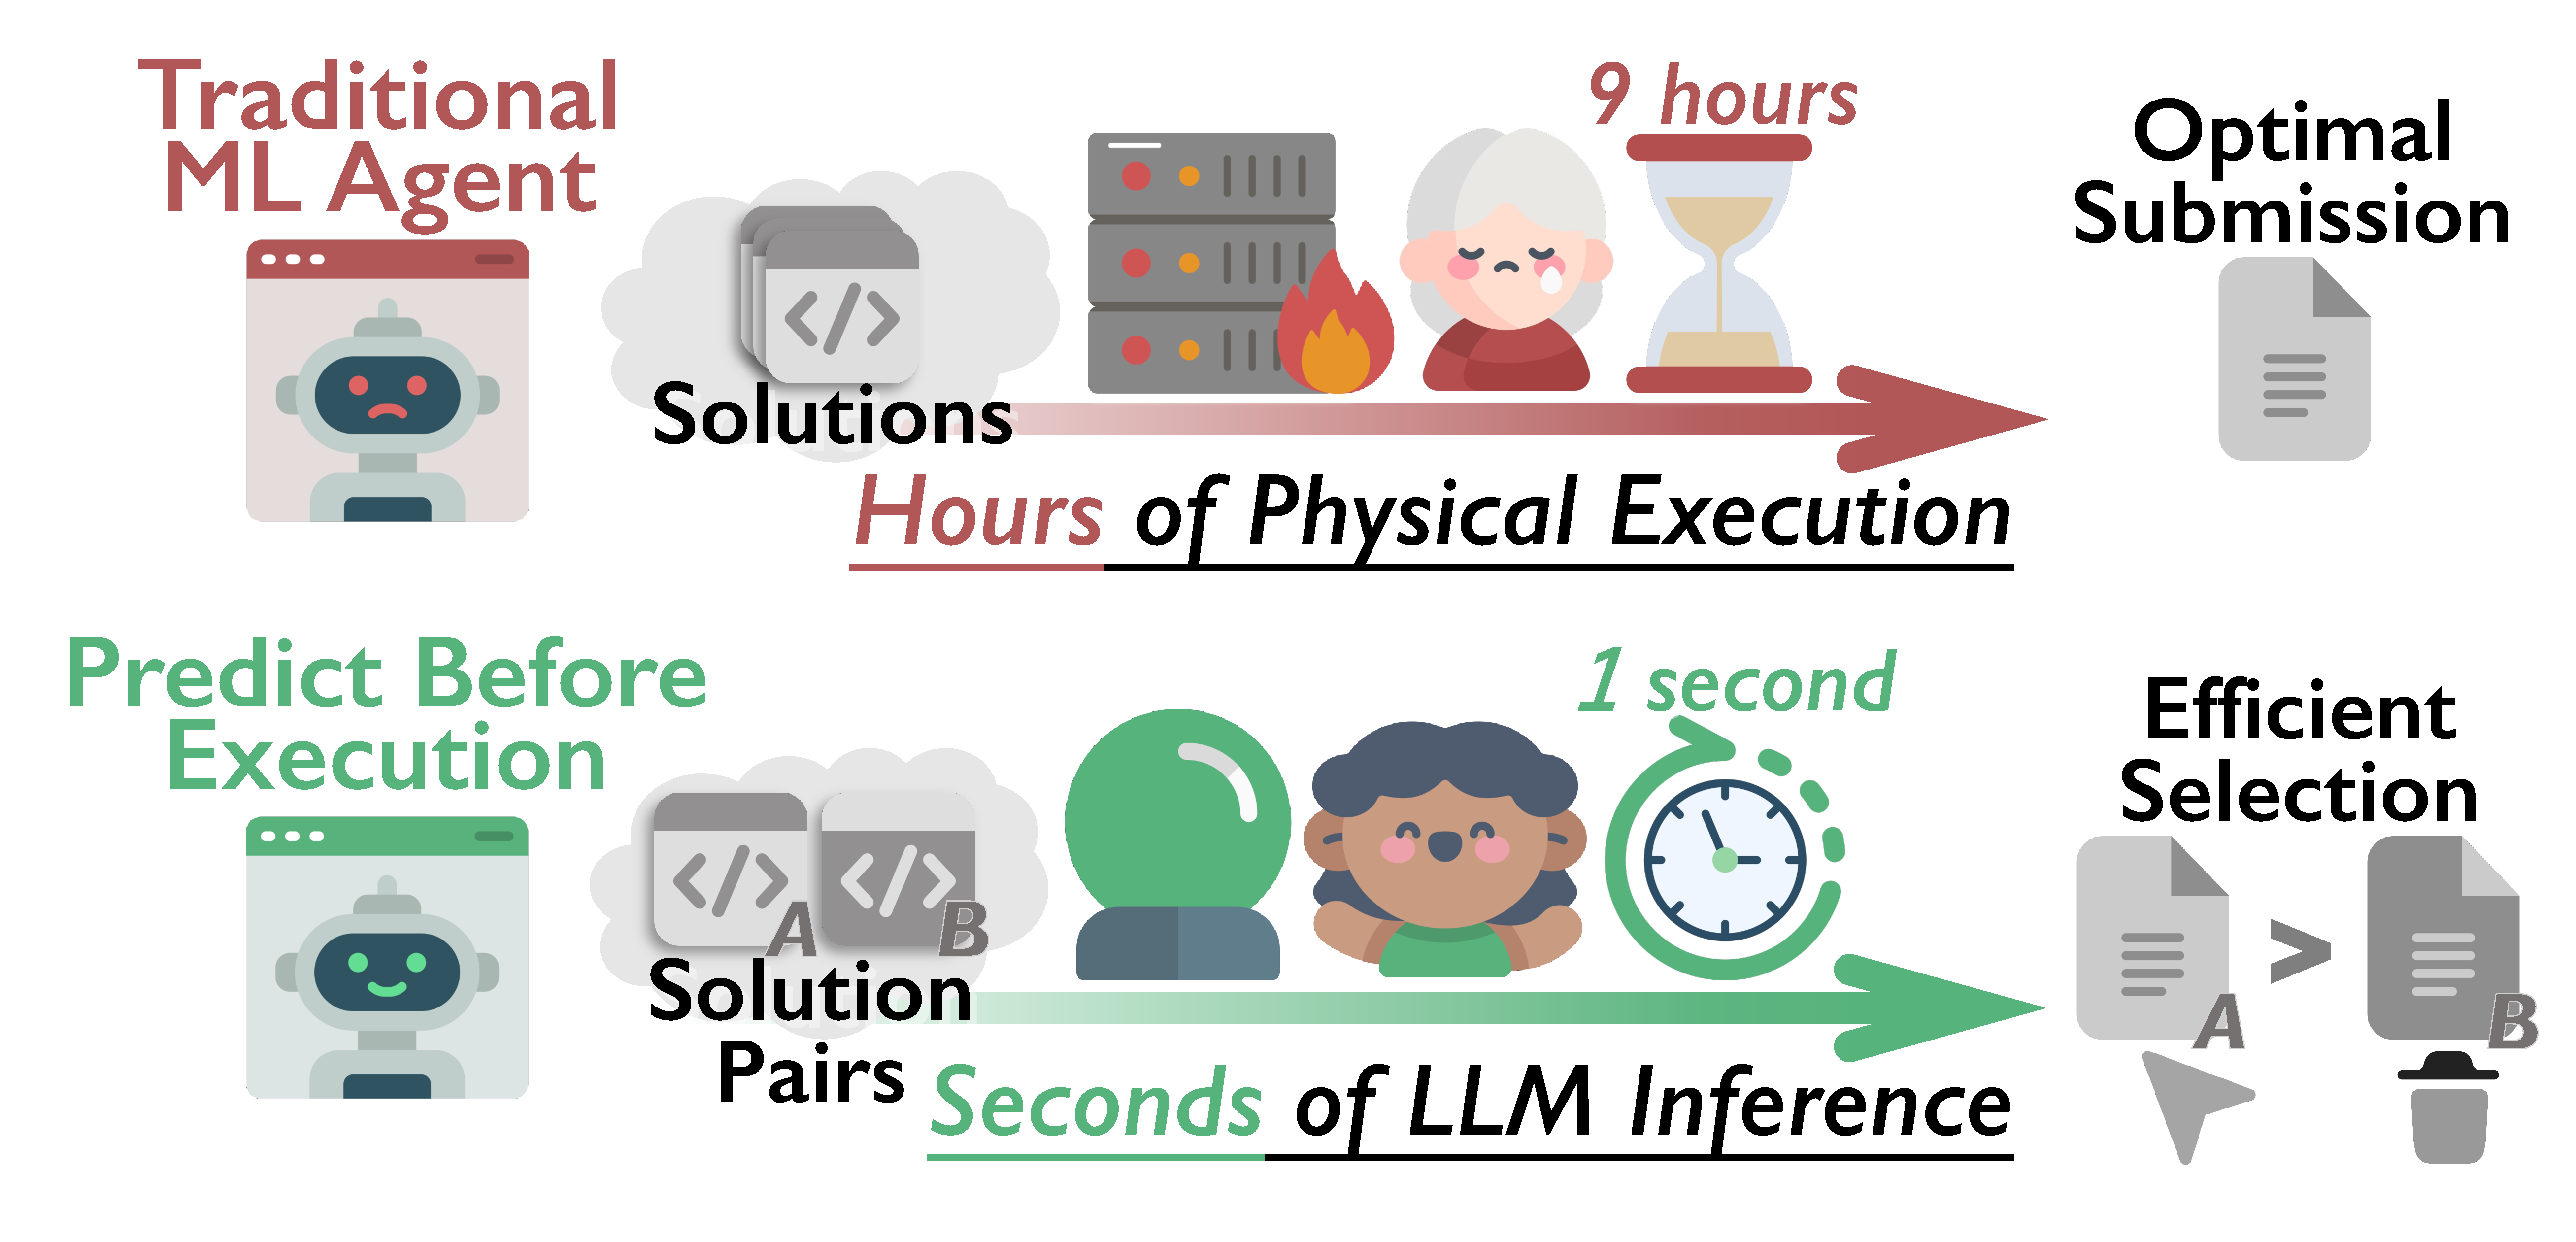
\includegraphics[width=1\linewidth]{figures/top.pdf}
    \caption{\textbf{From Execution to Inference.}
    Traditional ML agents improve through costly execution and external feedback, incurring substantial latency. 
    Our work investigates whether superior data-grounded solutions can be identified before execution by leveraging ``Implicit Execution Priors''.}
    \label{fig:top_concept}
\end{figure}

% Paragraph 2: Inspiration (Refined Logic)
To fundamentally bypass these physical constraints, the concept of \textbf{World Models}~\cite{Ding2025} offers a transformative alternative (Figure~\ref{fig:top_concept}).
Originating from reinforcement learning, world models enable agents to simulate environmental dynamics and evaluate actions via internal predictions rather than external trials~\cite{ha2018worldmodels, hafner2024masteringdiversedomainsworld}.
Recent advancements have extended this capability to the code domain by predicting execution outputs directly~\cite{li2025codeiocondensingreasoningpatterns, faircodegenteam2025cwmopenweightsllmresearch}.
Motivated by this, we explore whether agents can internalize execution priors, substituting costly runtime checks with instantaneous predictive reasoning.
The potential to replace \textbf{9 hours} of physical latency with \textbf{1 second} of neural speed brings us to a fundamental question: 
\textbf{\textit{Can we compress hours of physical execution into seconds of logical inference?}}

% Paragraph 3: Task Formulation, Main Results, and Mechanistic Insights
To answer this question, we formalize the task of \textbf{Data-centric Solution Preference}, where the model must predict the relative performance of two algorithmic solutions given a data analysis report, through reasoning without physical execution.
To rigorously evaluate this, we construct a large-scale corpus comprising 18,438 pairwise comparisons.
Our main experiments yield strong evidence: \textbf{LLMs exhibit significant predictive capabilities}, with DeepSeek-V3.2-Thinking achieving 61.5\% accuracy, outperforming both random guessing (50.0\%) and complexity-based heuristics (50.8\%).
Further analysis reveals that reasoning-optimized architectures transcend complexity heuristics through genuine data reasoning, yielding well-calibrated confidence that ensures the reliability of implicit evaluation.
Finally, we integrate this predictive mechanism into \textbf{\ours}, an agent that employs a \textit{Predict-then-Verify} loop to decouple exploration from execution, expanding the search space by $3.2\times$ and achieving a $6\times$ acceleration while delivering a +6\% performance gain over standard baselines.

% Paragraph 4: Contributions (Structured)
In summary, our contributions are three-fold:
\begin{itemize}
    \item We define the novel task of \textbf{Data-centric Solution Preference} and construct a comprehensive corpus of 18,438 pairs, answering the titular question that \textbf{LLMs Exhibit Significant Predictive Capabilities.}
    \item We operationalize this framework in \textbf{\ours}, an agent that employs a \textit{Predict-then-Verify} loop to decouple exploration from execution, enabling it to expand the search space by $\bm{3.2\times}$ and achieve a $\bm{6\times}$ acceleration and a \textbf{+6\%} performance gain over the baseline.
    \item We contribute a large-scale \textbf{Open-Source Dataset} of verified execution trajectories, serving as a foundational corpus for training scalable Reward Models to accelerate reinforcement learning rollouts and optimization across diverse agent frameworks.
\end{itemize}


\begin{figure*}[t]
    \centering
    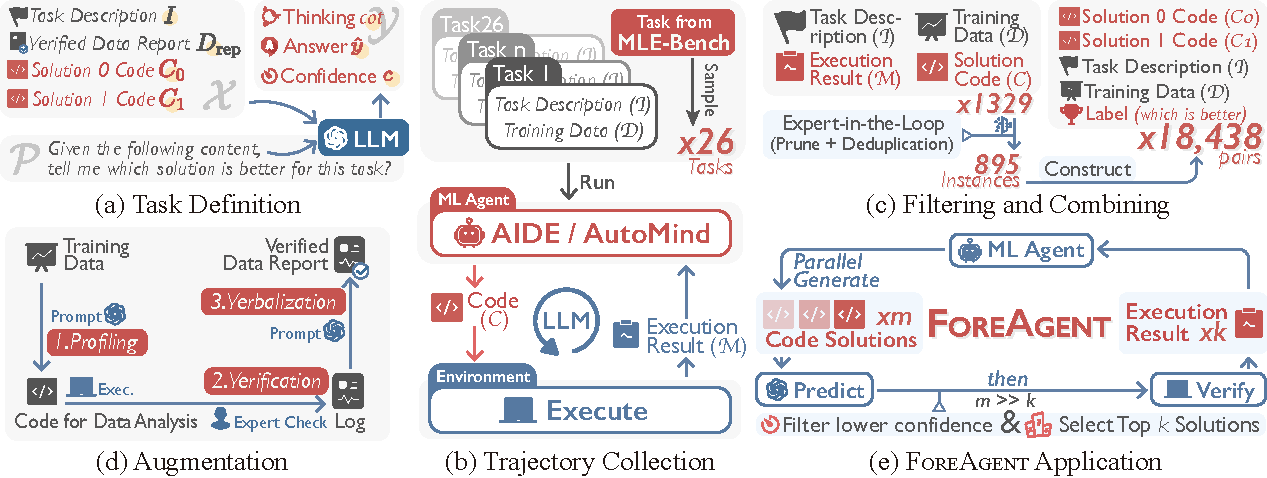
\includegraphics[width=\linewidth]{figures/main-v5.pdf}
    \caption{\textbf{Overview of the Framework.} \textbf{(a) Task Definition:} The \textit{Data-centric Solution Preference} task predicts solution superiority and confidence via latent reasoning. \textbf{(b-c) Data Curation:} We collect and filter real-world agent trajectories to construct the \textit{Preference Corpus}. \textbf{(d) Augmentation:} Inputs are augmented with \textit{Verified Data Reports} via a ``Profile-Verify-Verbalize'' pipeline. \textbf{(e) \ours Application:} The model serves as a filter within the \textit{Predict-then-Verify} loop, predicting preference \textit{before} physical execution to prune candidates.}
    \label{fig:main}
\end{figure*}